
\tableofcontents
\newpage

%%%%%%%%%%%%%%%%%%%%%%
%%%%%%%%% Capítulo I
%%%%%%%%%%%%%%%%%%%%%%%

\section{Planteamiento del problema}

%%%%%%%%% sección 1.1

\subsection{Situación problemática}
\parindent=12.7mm Los errores refractivos explican más de la mitad de las bajas visiones y cegueras en el mundo. En Australia los vicios de refracción dan cuenta del 62$\%$ de las personas con baja visión y 4$\%$ de las personas con ceguera \citep{Taylor_2005}. Según la oficina del censo de Estados Unidos indica que aproximadamente el 24$\%$ de la población son miopes y se estima que 43 millones de estos son candidatos para cirugía refractiva, aproximadamente el 26$\%$ de la población son hipermétropes de los cuales se estima que solo 15 millones de estos son candidatos para cirugía refractiva \citep{lombardo2014demographics}. La Organización Mundial de la Salud ha estimado que el vicio de refracción no corregido es responsable de baja visión en 153 millones de personas, y de ceguera en 5 millones de personas en el mundo.

Según el artículo de revisión ''Discapacidad visual en el Perú y su posible asociación con determinantes sociales de la salud'' \citep{bernuy2022discvisual}. Se trata de exponer las frecuencias de patologías oculares a nivel nacional y su relación con los determinantes sociales de la salud (DSS) de los cuales se encontraron que las patologías mas frecuentes son defectos de refracción y catarata, el cual afecta principalmente a los grupos etarios de 30-39 años y mayores de 60 años respectivamente. De los cuales por el reporte del MINSA en el 2018 se reportaron los siguientes casos en Perú y en el Cusco.

\begin{enumerate}
    \item \textbf{Perú:}
    \begin{itemize}
        \item \textbf{Catarata: }93934 casos
        \item \textbf{Glaucoma: }51581 casos
        \item \textbf{Ametropía: }79473 casos
        \item \textbf{Retina diabética: }8290 casos
        \item \textbf{DMRE: }8237 casos
        \item \textbf{ROP: }1507 casos
        \item \textbf{Trauma Oc: }11257 casos 
    \end{itemize}
    \item \textbf{Cusco:}
    \begin{itemize}
        \item \textbf{Catarata: }2512 casos
        \item \textbf{Glaucoma: }593 casos
        \item \textbf{Ametropía: }1750 casos
        \item \textbf{Retina diabética: }86 casos
        \item \textbf{DMRE: }168 casos
        \item \textbf{ROP: }16 casos
        \item \textbf{Trauma Oc: }692 casos 
    \end{itemize}
\end{enumerate}
En el que la Catarata y Ametropía (defecto de refracción) son los diagnósticos más comunes. Entonces viendo estos problemas en la población es necesaria su atención oportuna, diagnóstico y descarte de dichas enfermedades.

La cirugía refractiva se ha constituido como una desafiante subespecialidad de la Oftalmología corrigiendo los vicios de refracción. Pacientes con miopía, hipermetropía y astigmatismo, han logrado excelentes resultados en eficacia, estabilidad y seguridad; logrando reducir la dependencia de anteojos y lentes de contacto. Las técnicas más utilizadas son las queratorefractivas con láser excimer, especialmente la queratomileusis in situ con láser (LASIK) y la queratectomía fotorefractiva (PRK). Ambas dominando el tratamiento quirúrgico para ametropías bajas y moderadas. \citep{Ren_Moreno_2010}

El Laser In Situ Keratomileusis (LASIK) es un procedimiento quirúrgico para corregir miopía, hipermetropía y astigmatismo mediante ablación del estroma corneal. Que es realizada en dos partes: la creación del colgajo corneal y, seguido, la fotoablación con láser Excimer sobre el estroma corneal, reduciendo su espesor y modificando su curvatura \citep{sanchez2012cirugia}. Pese a su buena fama, la cirugía refractiva LASIK no está excenta de complicaciones y riesgos, aun que estos se den en muy bajos números el cual mediante algoritmos en el láser Excimer, la sobrecorrección ocurre raramente tras la aplicación de LASIK aunque estas hipocorrecciones o regresiones en pacientes específicos resulta inevitable.

Factores asociados a la regresión en LASIK y que requieren retratamiento no están definidos aunque estudios indican que puede ser causada por memoria ocular en las fibras de colágeno corneales, remodelamiento corneal, influencia de la presión intraocular (PIO) en la zona con menor espesor corneal y por hiperplasia del epitelio en respuesta a una excesiva curvatura plana corneal. Es necesario y útil en muchos casos realizar una mejora para refinar los resultados obtenidos tras la cirugía original, Retratamiento LASIK actúa sobre el estroma corneal, separando el flap original en la cual se aplica una segunda ablación.

Estudios como \citep{pravato2009inc} indicaron que la incidencia a retratamientos de cirugía LASIK se encuentra entre un 5$\%$ - $30\%$, otro autor como \citep{Hersh_2003} indica que la incidencia al retratamiento LASIK es mayor cuando la corrección de miopía y astigmatismo es alta además de que pacientes mayores también tienen mayor incidencia a necesitar un retratamiento LASIK. Esta frecuencia sigue representando un porcentaje de casos de pacientes insatisfechos, que deben ser sometidos a nueva cirugía asumiendo un nuevo riesgo, aunque sea pequeño.

\citep{Hettinger_2009} en su trabajo ``El rol de la bioestadística en la mejora de la calidad de la cirugía refractiva'' concluye que los análisis bioestadísticos ayudan a transformar las grandes cantidades de datos clínicos recopilados uniformemente disponibles para mejorar la práctica clínica. Los procesos de mejora basados en datos desempeñan un rol importante en la mejora de los resultados de los pacientes.

Entonces el presente trabajo evalúa el perfil de los pacientes sometidos a cirugía refractiva LASIK mediante el análisis de componentes principales, evaluar la prevalencia de retratamientos LASIK en la población evaluada y por último ver como se asocian estos componentes al retratamiento LASIK.

%%%%%%%%% sección 1.2

\subsection{Formulación del problema}
\subsubsection{Problema general}
¿Existe asociación entre el perfil composicional de pacientes sometidos para cirugía refractiva Laser In Situ Keratomileusis con respecto a ser sometido a un Retratamiento LASIK?
 
\subsubsection{Problemas específicos}

\begin{enumerate}

	\item ¿Qué variables estan asociadas al riesgo de poder realizarse un Retratamiento LASIK en pacientes sometidos a cirugía refractiva LASIK?
 
	\item ¿Podrán describir los componentes las características clínicas y demográficas en las pruebas preoperatorias de pacientes sometidos a cirugía refractiva LASIK?

    \item ¿Cómo afectan estos componentes en la predicción de realizarse un retratamiento LASIK?

\end{enumerate}

%%%%%%%%% sección 1.3

\subsection{Justificación de la investigación}
El estudio aplica técnicas bioestadística como el análisis de componentes principales de tal forma que pueda explicar las variables clínicas de pacientes sometidos a cirugía refractiva Laser In Situ Keratomileusis y ver su asociación en la incidencia de tener un retratamiento LASIK. De tal forma que nuevos estudios tomen en cuenta la importancia de las técnicas bioestadísticas que se puedan emplear en la cirugía refractiva ya sea para la predicción preoperatorio si un paciente tendrá la probabilidad de desarrollar un Retratamiento LASIK así como la influencia que tenga para el desarrollo de nomogramas posteriores.
 
%%%%%%%%% sección 1.4

\subsection{Objetivos de la investigación}

\subsubsection{Objetivo general}
Establecer si existe asociación entre el perfil composicional de pacientes sometidos para cirugía refractiva Laser In Situ Keratomileusis con respecto a ser sometido a un Retratamiento LASIK.

\subsubsection{Objetivos específicos}
\begin{enumerate}
\item 	Identificar variables y factores asociados al riesgo de poder realizarse un Retratamiento LASIK en pacientes sometidos a cirugía refractiva LASIK.
\item   Interpretar los componentes con respecto a sus variables originales de pacientes sometidos a cirugía refractiva LASIK.
\item Evaluar la asociación de componentes con respecto al Retratamiento LASIK.
\end{enumerate}


%%%%%%%%%%%%%%%%%%%%%%%%%%%%%%
%%%%%%%%%%%%%%%%%%% CAPÍTULO II
%%%%%%%%%%%%%%%%%%%%%%%%%%%%%%%%

\section{Marco teórico conceptual}

%\textbf{ Cómo hacer el marco teórico}

%En la elaboración del marco teórico se debe redactar un escrito con coherencia, secuencialidad y lógica. Utilizando citas de teorías o trabajos anteriores que sirvan de sustento al trabajo de investigación.
%
%Define los conceptos que se utilizaran, las variables, el enfoque de la investigación, resultados  obtenidos en investigaciones similares, de tal manera que cualquier persona que lea el marco conceptual pueda introducirse en el problema de investigación y además sea capaz de  comprenderlo sin dificultad.

%%%%%%%%% sección 2.1

\subsection{Bases teóricas}
\subsubsection{Conceptos básicos }

\begin{defi}\citep{Blyth_2002}
    Si se tiene $m$ y $n$ como números enteros positivos. Decimos a una \textbf{matriz de tamaño} $m$ por $n$, o una \textbf{matriz} $mxn$, como un arreglo con $mn$ números agrupados en $m$ filas y $n$ columnas, expresado en la siguiente manera

    $$
    \begin{bmatrix}
        X_{11} & X_{12} & X_{13} & \cdots & X_{1n} \\
        X_{21} & X_{22} & X_{23} & \cdots & X_{2n} \\
        X_{31} & X_{32} & X_{33} & \cdots & X_{3n} \\
        \vdots & \vdots & \vdots & \ddots & \vdots \\
        X_{m1} & X_{m2} & X_{m3} & \cdots & X_{mn}
    \end{bmatrix}
    $$

    Donde el primer sufijo representa a la \textbf{fila} y el segundo sufijo representa a la \textbf{columna}, tal que $x_{ij}$ aparece en la $i$-\'esima fila y la $j$-\'esima columna. De forma abreviada se tiene:
    $$X={\left[x_{ij} \right]}_{mxn}$$
    Donde $X$ es la matriz de tamaño $mxn$  donde $x_{ij}$ es el $(i,j)$-elemento o la $(i,j)$-entrada de la matriz.

\end{defi}

\begin{defi}\citep{Blyth_2002}
    Sea $A={\left[a_{ij} \right]}_{mxn}$ y $B={\left[b_{ij} \right]}_{nxp}$. Se define al \textbf{producto} $AB$ a la matriz $mxp$ donde el $(i,j)$-ésimo elemento es:
    $${\left[AB \right]}_{ij}=a_{i1}b_{1j}+a_{i2}b_{2j}+a_{i3}b_{3j}+\cdots+a_{in}b_{nj}$$ 
    Es decir que los $(i,j)$ elementos del producto $AB$ es obtenido por la suma de productos de los elementos de la $i$-\'esima fila de $A$ con los correspondientes elementos de la $j$\'esima columna de $B$, expresado también como la siguiente sumatoria:
    $${\left[AB \right]}_{ij}=\sum\limits_{k = 1}^{n}a_{ik}b_{kj}$$
\end{defi}

\begin{defi}\citep{Blyth_2002}
    Una matriz es llamada $cuadrada$ si el tamaño es $nxn$ es decir que tiene el mismo número de filas y columnas
\end{defi}

\begin{defi}\citep{Blyth_2002}
    Para cada matriz $A_{nxn}$ existe una única matriz $I_{n}$ de tamaño $nxn$ tal que $AI=A=IA$ llamada como \textbf{matriz identidad}  
\end{defi}

\begin{defi}\citep{Blyth_2002}
    Si $A$ es una matriz $mxn$, se llama \textbf{matriz transpuesta} a una matriz $A^T$ donde el $(i,j)$-\'esimo elemento es el $(j,i)$-\'esimo elemento de $A$. Mas precisamente decir si $A={\left[a_{ij} \right]}_{mxn}$ entonces $A^T={\left[a_{ji} \right]}_{nxm}$    
\end{defi}

\begin{defi}\citep{Blyth_2002}
    Una matriz $A_{nxn}$ es llamado \textbf{ortogonal} si:
    $$AA^T=I_n=A^TA$$    
\end{defi}

\begin{defi}\citep{Blyth_2002}
    Se entiende como \textbf{sistema de $m$ ecuaciones lineales con las $n$ incógnitas} $x_1,\cdots,x_n$ tal que la lista de ecuaciones se encuentra de la forma:
    \begin{align*}
a_{11}x_1 + a_{12}x_2 + a_{13}x_3 + \cdots + a_{1n}x_n &= b_1 \\
a_{21}x_1 + a_{22}x_2 + a_{23}x_3 + \cdots + a_{2n}x_n &= b_2 \\
a_{31}x_1 + a_{32}x_2 + a_{33}x_3 + \cdots + a_{3n}x_n &= b_3 \\
\vdots \quad \quad \quad \quad \quad \quad \quad \quad \quad \quad \quad \quad \\
a_{m1}x_1 + a_{m2}x_2 + a_{m3}x_3 + \cdots + a_{mn}x_n &= b_m
\end{align*}
Donde los $a_{ij}$ y los $b_i$ son números, expresados también de la siguiente forma:

$$\begin{bmatrix}
a_{11} & a_{12} & a_{13} & \cdots & a_{1n} \\
a_{21} & a_{22} & a_{23} & \cdots & a_{2n} \\
a_{31} & a_{32} & a_{33} & \cdots & a_{3n} \\
\vdots & \vdots & \vdots & \ddots & \vdots \\
a_{m1} & a_{m2} & a_{m3} & \cdots & a_{mn}
\end{bmatrix}
\begin{bmatrix}
x_1 \\
x_2 \\
x_3 \\
\vdots \\
x_n
\end{bmatrix}
=
\begin{bmatrix}
a_{11}x_1 + a_{12}x_2 + a_{13}x_3 + \cdots + a_{1n}x_n \\
a_{21}x_1 + a_{22}x_2 + a_{23}x_3 + \cdots + a_{2n}x_n \\
a_{31}x_1 + a_{32}x_2 + a_{33}x_3 + \cdots + a_{3n}x_n \\
\vdots \\
a_{m1}x_1 + a_{m2}x_2 + a_{m3}x_3 + \cdots + a_{mn}x_n
\end{bmatrix}$$
Donde se observa un sistema expresado de la forma matricial como $\mathbf{Ax=b}$ donde $A={\left[a_{ij} \right]}_{mxn}$ y $\mathbf{x,b}$ son las siguientes matrices columnas

$$\mathbf{x} =
\begin{bmatrix}
x_1 \\
x_2 \\
\vdots \\
x_n
\end{bmatrix}
, \quad
\mathbf{b} =
\begin{bmatrix}
b_1 \\
b_2 \\
\vdots \\
b_m
\end{bmatrix}$$
La matriz $A_{mxn}$ es llamada \textbf{matriz de coeficientes} del sistema.
\end{defi}

\begin{defi}\citep{Blyth_2002}
    Sea una matriz $A_{mxn}$ es llamado \textbf{matriz inversa izquierda de} $A$ a una matriz $X_{nxm}$ si satisface la ecuación $XA=I_n$; y una \textbf{matriz inversa derecha de} $A$ si satisface la ecuación $AX=I_m$
\end{defi}

\begin{defi}\citep{Blyth_2002}
    Un \textbf{espacio vectorial} es un conjunto $V$ de $F$ en el cual se definen dos operaciones ``adición'' y ``multiplicación de escalares''. Si los escalares son números reales sería un \textbf{espacio vectorial real}, y si los escalares son números complejos sería un \textbf{espacio vectorial complejo}. Por lo tanto $F$ puede pertenecer a los números reales o los números complejos.
\end{defi}

\begin{defi}\citep{Blyth_2002}
    Si $V$ y $W$ son espacios vectoriales sobre un cuerpo $F$ entonces por \textbf{aplicación lineal} (o \textbf{transformación lineal}) de $V$ a $W$ nos referimos a una aplicación $f: V \to W $ tal que
    \begin{enumerate}
        \item $(\forall x,y \in V) \quad f(x+y)=f(x)+f(y)$
        \item $(\forall x \in V)(\forall \lambda \in F) \quad f(\lambda x)=\lambda f(x)$ 
    \end{enumerate}
\end{defi}

\begin{defi}\citep{Blyth_2002}
    Un \textbf{autovalor} (o \textbf{valor latente}) de $A$ es un escalar $\lambda$ para el que existe una matriz no cero $\mathbf{x}_{nx1}$ tal que $X\mathbf{x}=\lambda \mathbf{x}$. Tal que las columnas de la matriz $\mathbf{x}$ son llamados \textbf{autovectores} (o \textbf{vectores latentes}) asociados con $\lambda$
\end{defi}

\subsubsection{Análisis de componentes principales}
\citep{aldas2017analisis} El análisis de componentes principales (PCA) toma las variables incorrelacionadas entre sí y que puedan ordenarse de acuerdo con la información que llevan incorporada para crear nuevas variables llamadas componentes.

\begin{enumerate}
    \item \textbf{Componentes principales de dos variables:} Tomemos en cuenta que se tienen dos variables distribuidas normalmente y que están correlacionadas entre sí, de tal forma que su gráfico de dispersión formará una elipse como se muestra en la figura \ref{fig:autovec_autova_2dim}. En la cual se pueda trazar dos líneas perpendiculares que midan la longitud y la altura de la elipse. Estas líneas vienen a ser los autovectores de la matriz de correlaciones, además de que las líneas al ser perpendiculares vienen a ser los autovectores. Si se añadiera una tercera variable la elipse se convertiría en un balón de rugby y se tendrían tres lineas perpendiculares, tres autovectores y así sucesivamente.

    \begin{figure}[htb]
    \centering
    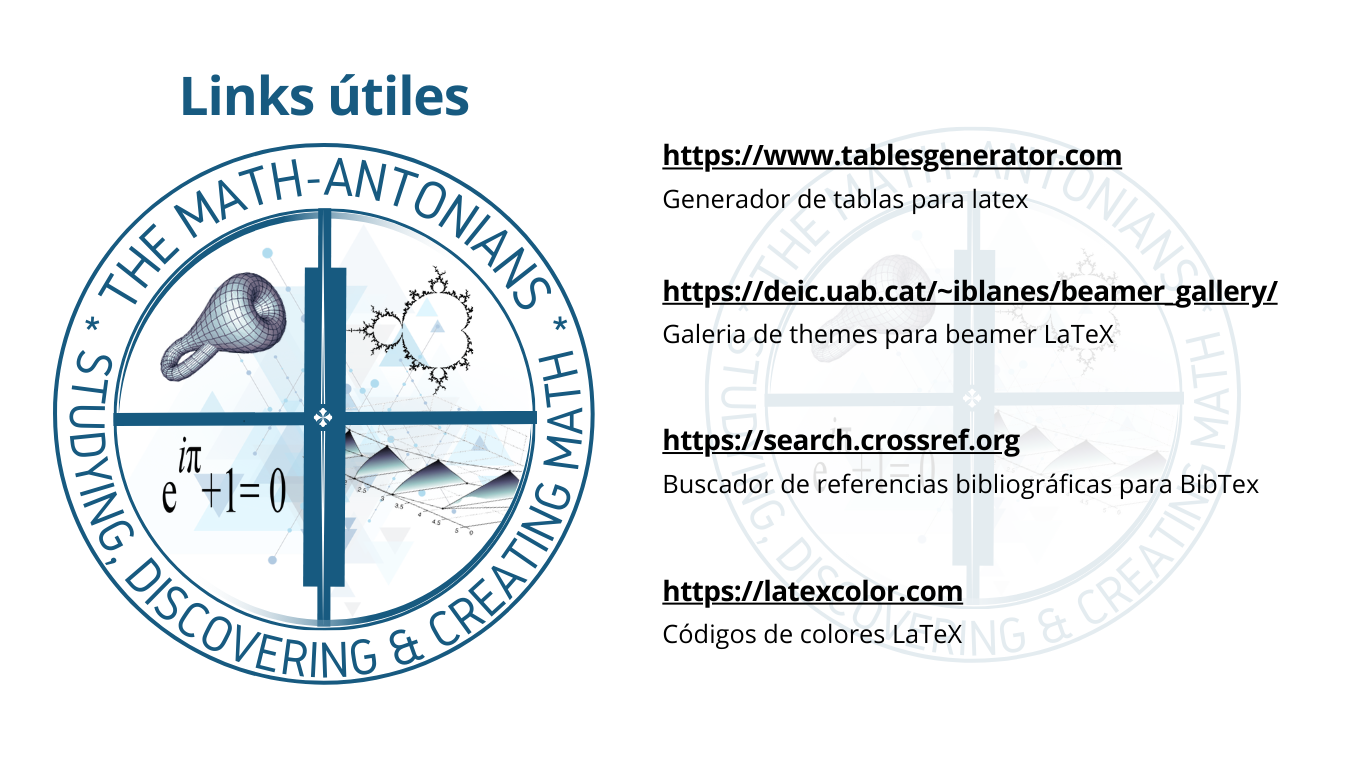
\includegraphics[scale=0.75]{imagenes/001.png}
    \caption{Interpretación gráfica de autovectores y autovalores \citep{aldas2017analisis}}
    \label{fig:autovec_autova_2dim}
    \end{figure}

    Cada autovector tienen un asociado un autovalor. El autovalor da una medida de longitud del autovector y observando ese valor se puede ver si los datos están distribuidos de forma homogénea o heterogénea. Entonces se parte de la matriz de correlaciones en el cual se muestra que existe un nivel de correlación razonable entre las variables que justifique el uso de un PCA.

    Si tomamos en cuenta los autovectores calculados se tendría la siguiente matriz:

    $$\mathbf{u}_1 = \begin{bmatrix} u_{11} \\ u_{12} \end{bmatrix} ; \mathbf{u}_2 = \begin{bmatrix} u_{21} \\ u_{22} \end{bmatrix}$$


    La aplicación del procedimiento de componentes principales requiere calcular los autovalores y autovectores de la matriz de covarianzas. En el cual los autovectores representan el giro que se ha producido entre los ejes. Así genéricamente se tiene que aplicar a las variables originales los coeficientes de vectores $\mathbf{u}_1$ y $\mathbf{u}_2$ expresados de la siguiente manera:
    $${x}_{1}^{*}={u}_{11}X_1+{u}_{12}X_2$$
    $${x}_{2}^{*}={u}_{21}X_1+{u}_{22}X_2$$

    Así mismo deben de cumplir las condiciones arbitrarias pero necesarias de que los ejes sean ortogonales \eqref{eq:ort} y fijar las escalas de medida \eqref{eq:medi}
    \begin{equation}
    u_{11}^2 + u_{12}^2 = 1 \quad ; \quad u_{21}^2 + u_{22}^2 = 1
    \label{eq:ort}
    \end{equation}
    \begin{equation}
    u_{11}u_{21} + u_{21}u_{22}=0 
    \label{eq:medi}
    \end{equation}
    En el análisis de componentes principales es importante conocer la correlación de cada variable con las componentes para tener una medida de lo importante que es cada variable en la interpretación del compoente principal. A este se le denomina \textbf{carga factorial} $l_{hj}$ entre la componente $h$-\'esima y la variable $j$-\'esima viene dada por:

    \begin{equation}
    l_{hj} = \frac{u_{hj}}{\hat{s_j}}\sqrt{{\lambda}_{h}}}
    \label{eq:car_fac}
    \end{equation}

    Donde la única notación no conocida es $\hat{s_j}$ que viene a ser la desviación típica de la variable $j$-\'esima

    \item \textbf{Componentes principales para el caso general:} La obtención de componentes principales es un caso típico de cálculo de autovalores y autovectores de una matriz simétrica.

    \begin{enumerate}
        \item \textbf{Obtención de la primera componente} Considere que se dispone de una muestra de tamaño $n$ acerca de las $p$ siguientes variables $X_1,X_2,\ldots,X_p$ y que las observaciones están expresadas bien en desviaciones respecto a la media (centradas) o bien como variables tipificadas. La primera componente, de la misma forma que el resto, se expresa como combinación lineal de las variables originales:

        \begin{equation}
        Z_{1i} = u_{11}X_{1i} + u_{12}X_{2i} + \ldots + u_{1p}X_{pi}
        \label{eq:comb_lina_comp}
        \end{equation}

        Puede comprobarse fácilmente que tanto si las $X_j$ variables están expresadas en desviaciones como si están tipificadas se obtiene que la media muestral de $Z_1$ es igual a $0$.
        Para el conjunto de las $n$ observaciones muestrales esta ecuación se puede expresar matricialmente de la siguiente forma:

        \begin{equation}
        \begin{bmatrix}
        Z_{11} \\
        Z_{12} \\
        \vdots \\
        Z_{1n}
        \end{bmatrix}
        =
        \begin{bmatrix}
        X_{11} & X_{21} & \cdots & X_{p1} \\
        X_{12} & X_{22} & \cdots & X_{p2} \\
        \vdots & \vdots & \ddots & \vdots \\
        X_{1n} & X_{2n} & \cdots & X_{pn}
        \end{bmatrix}
        \begin{bmatrix}
        u_{11} \\
        u_{12} \\
        \vdots \\
        u_{1p}
        \end{bmatrix}
        \label{eq:comp_matriz}
        \end{equation}
        o en notación matricial compacta:
        \begin{equation}
            \mathbf{z_1}=\mathbf{Xu_1}
            \label{eq:comp_lineal}
        \end{equation}
        La primera componente se obtiene de forma que su varianza sea máxima, sujeta a la restricción de que la suma de los pesos $u_{ij}$ al cuadrado sea igual a la unidad. La varianza del primer componente, teniendo en cuenta que su media es 0, vedrá dada por:
        \begin{equation}
            var(Z_1)=\frac{\sum\limits_{i = 1}^{n}{Z}_{1j}^{2}}{n}=\frac{1}{n}\mathbf{{z}_{1}'{z}_{1}}=\frac{1}{n}\mathbf{{u}_{1}'X'Xu_1}=\mathbf{u_{1}'} \left[ \frac{1}{n} \mathbf{X'X} \right] \mathbf{u_{1}}}
            \label{eq:var_matriz}
        \end{equation}
        Si las variables están expresadas en desviaciones respecto a la media, $(1/n)\mathbf{X'X}$ es la matriz de covarianzas muestral a la que denominaremos $\mathbf{V}$; para variables tipificadas $(1/n)\mathbf{X'X}$ es igual a la matriz de correlaciones $\mathbf{R}$. Las componentes pueden obtenerse para ambos tipos de variables, aunque en los paquetes de ordenador para análisis multivariante se utiliza la matriz de correlación en la mayor parte de los casos. A efectos expositivos y para darle mayor generalidad vamos a suponer, sin embargo, que utilizamos la matriz de covarianzas. Por lo tanto, la varianza a maximizar es:
        \begin{equation}
            var(Z_1)=\mathbf{u_1'Vu_1}
            \label{eq:var_matriz}
        \end{equation}
        La restricción señalada analíticamente de que la suma de los cuadrados de los pesos sea la unidad viene dada por:
        \begin{equation}
            \sum\limits_{j = 1}^{p}{u}_{1i}^{2}=\mathbf{u_1'u_1}=1
            \label{eq:sum_cuad}
        \end{equation}
        En consecuencia, incorporando esta restricción se forma el siguiente lagrangiano:
        \begin{equation}
            \mathbf{L}=\mathbf{u_1'Vu_1}-\lambda(\mathbf{u_1'u_1}-1)
        \end{equation}
        Para maximizar el valor lagrangiano derivamos respecto a $\mathbf{u_1}$ e igualmente a 0:
        \begin{equation}
            \frac{\partial \mathbf{L}}{\partial \mathbf{u_1}}=2V\mathbf{u_1}-2\lambda \mathbf{u_1}=\mathbf{0}
        \end{equation}
        es decir:
        \begin{equation}
            (\mathbf{V}-\lambda \mathbf{I})\mathbf{u_1}=\mathbf{0}
        \end{equation}
        Al resolver la ecuación $|\mathbf{V}-\lambda \mathbf{I}|=0$, se obtienen $p$ autovalores. Si se toma la raíz característica mayor ($\lambda_1$), se halla el autovector asociado a la misma $\mathbf{u_1}$, aplicando la regla de normalización dada en \eqref{eq:sum_cuad}. Así el vector de ponderaciones que se aplica a las variables iniciales para obtener la primera componente principal es el autovector asociado al mayor autovalor de la matriz $\mathbf{V}$.

        \item \textbf{Obtención de las restantes componentes} Una componente genérica expresada en forma matricial para todas las observaciones viene dada, de forma análoga a \eqref{eq:comp_lineal}, por:
        \begin{equation}
            \mathbf{z_h}=\mathbf{Xu_h}
            \label{eq:comp_lineal_res}
        \end{equation}
        Para su obtención, además de la restricción de:
        \begin{equation}
            \mathbf{u_h'u_h}=1
            \label{eq:restriccion}
        \end{equation}
        se imponen las restricciones adicionales ya expuestas de que:
        \begin{equation}
            \mathbf{u_h'u_1}=\mathbf{u_h'u_2}=\ldots=\mathbf{u_h'u_{h-1}=0}
            \label{eq:restriccion}
        \end{equation}
        Por lo tanto, se imponen las restricciones adicionales de que el vector característico asociado a la componente $h$-\'esima sea ortogonal a todos los vectores característicos calculados previamente. Su obtención, a parte de tener en cuenta las restricciones \eqref{eq:restriccion}, plante problemas conceptuales nuevos. En todo caso señalaremos que el vector $\mathbf{u_h}$ está asociado a la raíz $h$-\'esima, una vez ordenadas de mayor a menor. En definitiva, las $p$ componentes principales que se pueden calcular son una combinación lineal de las variables originales, en la que los coeficientes de ponderación son los correspondientes vectores característicos asociados a la matriz $\mathbf{V}$.
        \item \textbf{Varianzas de las componentes} Si se tienen en cuenta las propiedades de los autovalores y como ilustramos en el caso de dos componentes, la varianza de la componente $h$-\'esima coincide su autovalor, es decir:
        \begin{equation}
            Var(Z_h)=\mathbf{u_h'Vu_h}=\lambda_{h}
        \end{equation}
        Adoptando como medida la variabilidad de las variables originales la suma de sus varianzas, dicha variabilidad será igual a la traza de la matriz $\mathbf{V}$. Ahora bien, la traza de la matriz $\mathbf{V}$ se puede expresar así teniendo en cuenta:
        \begin{equation}
            \frac{\lambda_{h}}{traza\mathbf{V}}=\frac{\lambda_h}{\sum\limits_{h = 1}^{p}\lambda_h}
        \end{equation}
        y en el caso particular en los datos estuviera tipificados y la matriz de covarianzas fuera la de correlación $\mathbf{R}$, entonces dado que $traza(\mathbf{R})=p$, la proporción de variabilidad correspondiente a la componente $h$-\'esima es:
        \begin{equation}
            \frac{\lambda_h}{p}
        \end{equation}
        \item \textbf{Correlación entre las componentes principales y las variables originales:} Primeramente se debe calcular la covarianza entre la variable $X_j$ y el componente $Z_h$. Definamos los vectores muestrales de la componente $Z_h$ y variable $X_j$ por:
        \begin{equation}
            \mathbf{x_j}=
            \begin{bmatrix}
            X_{j1} \\
            X_{j2} \\
            \vdots \\
            X_{jn}
            \end{bmatrix}
            \quad
            \mathbf{z_h}=
            \begin{bmatrix}
            Z_{h1} \\
            Z_{h2} \\
            \vdots \\
            Z_{hn}
            \end{bmatrix}
        \end{equation}
        La covarianza muestral entre $X_j$ y $Z_h$ viene dada por:
        \begin{equation}
            cov(X_j,Z_h)=\frac{1}{n}\mathbf{x_j'z_h}
            \label{eq:covarianzas}
        \end{equation}
        El vector $\mathbf{x_j}$ se puede expresar en función de la matriz $\mathbf{X}$, utilizando el vector de orden $p$, al que designaremos por $\delta$, que tiene un 1 en la posición $j$-\'esima y 0 en las posiciones restantes. Así,
        \begin{equation}
            \mathbf{x_j'}=\mathbf{\delta'X}=\left[0\enspace \ldots \enspace 1\enspace \ldots \enspace 0 \right]
            \begin{bmatrix}
            X_{11} & \cdots & X_{1i} & \cdots & X_{1n} \\
            \vdots & \vdots & \vdots & \vdots & \vdots \\
            X_{j1} & \cdots & X_{ji} & \cdots & X_{jn} \\
            \vdots & \vdots & \vdots & \vdots & \vdots \\
            X_{p1} & \cdots & X_{pi} & \cdots & X_{pn}
        \end{bmatrix}
        \end{equation}
        Teniendo en cuenta la expresión anterior y \eqref{eq:comp_lineal_res}, la covarianza dada en \eqref{eq:covarianzas} puede expresarse de la siguiente forma:
        \begin{equation}
            cov(X_j,Z_h)=\frac{1}{n}\mathbf{\delta'X'Xu_h}=\mathbf{\delta'Vu_h}=\mathbf{\delta'}\lambda_h\mathbf{u_h}=\lambda_h\mathbf{\delta'u_h}=\lambda_hu_{hj}
        \end{equation}
        En consecuencia, la correlación existente entre la variable $X_j$ y la componente $Z_h$, que recordemos denominábamos \textbf{carga factorial}, es la siguiente:
        \begin{equation}
            l_{jh}=\frac{cov(X_j,Z_h)}{\sqrt{var(Xj)}\sqrt{var(Z_h)}}=\frac{\lambda_hu_{hj}}{\sqrt{var(X_j)}\sqrt{\lambda_h}}=\frac{u_{hj}}{\sqrt{var(X_j)}}\sqrt{\lambda_h}
        \end{equation}
        expresión que coincide con la que derivamos en su momento \eqref{eq:car_fac}. En el caso en que las variables estén tipificadas (varianza 1), la expresión anterior adopta la forma:
        \begin{equation}
            l_{hj}=u_{hj}\sqrt{\lambda_h}
        \end{equation}
        que es la que se corresponde con las llamadas \textsl{matrices factoriales} en la mayoría de programas estadísticos.
    \end{enumerate}
    \item \textbf{Número de componentes principales a extraer:} La decisión a tomar es cuánta información (varianza) estamos dispuestos a sacrificar para ganar facilidad de intepretación. Aunque depende del juicio del investigador, las reglas mostradas serán orientativas.
    \begin{enumerate}
        \item \textbf{Criterio del autovalor superior a la unidad:} El criterio de retener aquellas componentes cuyo autovalor sea superior a la unidad es la opción por defecto de la mayoría de programas estadísticos. Si una componente no es capaz de explicar más información que una variable, no va a facilitar la reducción de datos, es decir, facilitar la interpretabilidad de la información. El criterio planteado de manera general es retener aquellas componentes cuyos autovalores sean superiores a la media de los autovalores
        \begin{equation}
            \lambda_h>\bar{\lambda}=\frac{\sum\limits_{j = 1}^{p}\lambda_j}{p}
            \label{eq:criterio}   
        \end{equation} 
        pero, como cuando trabajamos con variables tipificadas, se verifica que la suma de los autovalores coincide con la matriz de correlaciones, que es $p$, entonces:
        \begin{equation}
            \sum\limits_{j = 1}^{p}\lambda_j=p
        \end{equation}
        por lo que el criterio \eqref{eq:criterio} se puede expresar como decíamos al principio:
        \begin{equation}
            \lambda_h>1
        \end{equation}
        Se demostró que el criterio funciona bastante bien salvo que se tenga un gran número de variables ($>40$) siendo especialmente preciso con un número pequeño de variables (10-15). La varianza de una variable explicada por el componente (comunalidad) también influye en la precisión del criterio.

        \item \textbf{Criterio del gráfico de sedimentación \textsl{(scree plot)}} En esta parte se propone representar en un gráfico los autovalores correspondientes a las distintas componentes. Como los autovalores siempre son decrecientes, lo será este gráfico de líneas. El criterio es retener aquellas componentes anteriores a donde la línea comienza a nivelarse (si fuera la ladera de una montaña y cayesen rocas, donde estas comenzarían a parse o sedimentar, de ahí el nombre del gráfico), aunque si no se usa con precaución se puede descartar componentes que pueden ser relativas en la revelancia teórica de las mismas.
        \begin{figure}[htb]
        \centering
        \includegraphics[scale=1]{imagenes/002.png}
        \caption{Gráfico de sedimentación \citep{aldas2017analisis}}
        \label{fig:sedimentacion2}
        \end{figure}

        \item \textbf{Método paralelo:} Es obvio que hay mucha subjetividad en decidir dónde se produce el ``codo'' en la línea que marcaría el corte, sobre todo cuando la caída es progresiva. En la figura \ref{fig:sedimentacion2} no tendríamos muy claro si considerar tres o cuatro componentes al menos. Por está razón Horn (1965)\footnote{A rationale and a test for the number of factors in factor analysis. \textsl{Psychometrika}, 30:179-185} sugirió un procedimiento llamado análisis paralelo para objetivar este criterio en el cual indica que cuando se tienen datos totalmente incorrelacionados, un PCA debería generar autovalores iguales a 1 (cada autovalor explica la varianza de una única variable). Sin embargo, los errores de muestreo generan correlaciones espúreas que hace que unos autovalores sean superiores a la unidad y otros inferiores. La estrategia de Horn es contrastar los autovalores obtenidos mediante un PCA paralelo aplicado a muestras aleatorias de variables no correlacionadas con el mismo número de variables y observaciones que la muestra original que generarán autovalores que se han ajustado para evitar el error muestral. Solo se retendría aquellas componentes con autovalores ajustados superiores a la unidad. El autovalor ajustado vendrá dado por la expresión:
        \begin{equation}
            \lambda_p-(\bar{\lambda_p^r}-1)
        \end{equation}
        donde $\lambda_p$ es el autovalor $p$-\'esimo de los datos originales y $\bar{\lambda_p^r}$ es la media de las estimaciones de ese mismo autovalor en las submuestras aleatorias generadas.
        \item \textbf{Test estadístico:} El test utilizado es el de Bartlett (1951)\footnote{The effect of standardization on a chi square. Aproximation in factor analysis. \textsl{Biometrika}, 38(3/4):337-344} para analizar si la matriz de correlaciones es la identidad, adolece de las mismas limitaciones - básicamente ser muy sensible al tamaño muestral - y no recomiendan su uso pues suele aconsejar la retención de demasiadas componentes principales. Se considera que los $p-m$ últimos autovalores poblacionales son iguales a 0. Si los autovalores muestrales que observamos correspondientes a estas componentes no son exactamente igual a 0, se debe a los problemas del azar. Por ello, bajo el supuesto de que las variables originales siguen una distribución normal multivariante, se pueden formular las siguientes hipótesis relativas a los autovalores poblacionales:
        \begin{equation}
            H_0:\lambda_{m+1}=\lambda_{m+2}=\ldots=\lambda_p=0
        \end{equation}
        El estadístico para el contraste de esta hipótesis es el siguiente
        \begin{equation}
            Q^*=\left\{n-\frac{2p+11}{6} \right\}\left\{(p-m)ln\bar{\lambda}_{p-m}-\sum\limits_{j = m+1}^{p}ln\lambda_j \right\}
        \end{equation}
        Bajo la hipótesis nula, el estadístico anterior se distribuye como una ji-cuadrado con ($p-m+2$)($p-m+1$)$/2$ grados de libertad. Existen algunas variantes de este test básicamente referidas al cálculo de los grados de libertad, como son las de Anderson (1963)\footnote{Asymptotic theory for principal component analysis. \textsl{Annals of Mathematical Statistics}, 34(1):122-148} y Lawley (1956)\footnote{Tests of significance for the latent roots of covariance and correlation matrix. \textsl{Biometrika}, 43(1/2):128-136}.
    \end{enumerate}
    \item \textbf{Interpretación de las componentes principales:} Para interpretar las dos componentes extraídas es necesario fijarse en la contribución de cada variable. Al trabajar con datos tipificados, los valores estandarizados (cargas) y sin estandarizar coinciden. Cuanto mayor es la carga, mayor es la influencia que ha tenido esa variable en la formación de la componente. Por lo tanto podemos analizar cuáles son las cargas más altas y usar las variables a las que corresponden para dar una interpretación al eje.
\end{enumerate}


%%%%%%%%% sección 2.2

\subsection{Marco conceptual}

Los siguientes conceptos se extraerán de \citep{sanchez2012cirugia}

\begin{itemize}
    \item \textbf{Cirugía refractiva: }La cirugía refractiva es una subespecialidad de la oftalmología que engloba diferentes tipos de procedimientos quirúrgicos (incisionales, fotoablativos y lenticulares) que producen la corrección de los defectos de refracción del ojo humano.

    \item \textbf{Fisiología óptica: }El segmento anterior del ojo está compuesto de una estructura óptica esencial para la visión:
    \begin{itemize}
        \item \textbf{La córnea: }Órgano avascular y transparente compuesto por cinco diferentes capas histológicas. La función primordial de la córnea  consiste en enfocar las imágenes provenientes del exterior sobre la porción neurosensorial del ojo.
        \item \textbf{La retina: }El desvío de los rayos luminosos que componen las imágenes hacia la retina se denomina refracción.
    \end{itemize}
    Cuando las imágenes proyectadas desde la parte anterior del ojo se forman exactamente sobre la retina, el individuo es capaz de percibir nítidamente estas imágenes: a esa condición se denomina \textbf{emetropía}. Sin embargo, cuando los rayos de luz se enfocan fuera de la retina, se produce un defecto en la percepción visual denominado \textbf{ametropía} o defecto refractivo.
    \begin{enumerate}
        \item \textbf{Miopía: }Ocurre cuando el ojo es demasiado largo y/o la curvatura de la córnea es demasiado curva. Las imágenes que entran al ojo miope se enfocan \textbf{delante de la retina}, de tal manera que se produce una visión borrosa o desenfocada de las mismas para la visión de lejos. En general, el paciente con miopía tiene una excelente visión de cerca.
        \item \textbf{Astigmatismo: }Ocurre cuando la córnea se curva más en una dirección que la otra. Es como si la superficie anterior del ojo pareciese una pelota de rugby en lugar de a una pelota de fútbol. Si el astigmatismo es significativo, las imágenes que llegan a la retina a partir de un objeto son \textbf{múltiples} y en \textbf{diferentes focos}, produciéndose una visión distorionada del objeto.
        \item \textbf{Hipermetropía: }Se produce cuando el ojo es corto y/o la curvatura corneal es muy plana. Las imágenes que entran al ojo se enfocan por detrás de la retina, de tal manera que se produce una visión borrosa o desenfocada de las mismas, sobre todo en la visión cercana, aunque en grados significativos de hipermetropía la visión lejana también puede estar afectada.
    \end{enumerate}  
    \item \textbf{Excimer Láser: }LASER es una abreviación que significa amplificación de la luz por emisión estimulada de radiación. Básicamente consiste en una fuente de radiación (sólida, líquida o gaseosa) que luego de ser estimulada apropiadamente emite una forma de energía luminosa que es amplificada y dirigida hacia el tejido blanco. De acuerdo al tipo de fuente de radiación usada se obtienen diferentes tipos de energía LASER, cada una de las cuales tienen un determinado efecto sobre el ojo; fotoablación, fotodisrupción o fotocoagulación. El término Excimer es una contracción de dímero excitado, una molécula energizada de dos componentes. El Excimer utiliza los gases del argón y del flúor para generar un haz de luz ultravioleta con una longitud de onda de 193 nm. La energía de esta longitud de onda de la luz es suficiente para romper los enlaces moleculares en la córnea y quitar una capa muy fina de tejido. Este proceso es denominado fotoablación\footnote{Azar Dimitri T. Refractive Surgery. Second edition. \textsl{Mosby Elseiver}, 2007}. La ablación de la córnea con el Excimer Láser produce que el retiro de entre 0.1 a 0.25 micras de tejido por cada aplicación, con mínimo o ningún daño al tejido circundante. Esta precisión submicrónica es la clave de la seguridad y eficacia obtenidas con este procedimiento. De esta manera, el Excimer Láser es capaz de moldear sobre la córnea, una nueva superficie refractiva, permitiendo de esta manera que las imágenes lleguen en forma precisa hasta los órganos sensoriales.
    \begin{itemize}
        \item \textbf{Fundamentos de la Cirugía Refractiva con Excimer Láser: }El objetivo de la cirugía refractiva es \textbf{\testsl{modificar la curvatura de la córnea,}} y así cambiar su poder de convergencia.
        Un ojo hipermétrope tiene un déficit de convergencia. Para incrementar la convergencia, es necesario aumentar la curvatura corneal en el centro, lo que se logra eliminando tejido en la periferia, en forma de anillo.
        Un ojo miope tiene un exceso de convergencia que para disminuirla, es necesario reducir la curvatura corneal, lo que se logra removiendo tejido en forma de círculo en el centro de la córnea.
        Un astigmatismo tendrá más poder de convergencia en un eje de la córnea. Para la corrección del astigmatismo se llevan a cabo diferentes ablaciones en la parte central como en la periferia de la córnea dando como resultado el aplanamiento del meridiano más curvo y el encurvamiento del meridiano más plano. 
    \end{itemize}
    \item \textbf{Evaluación preoperatoria: }Al ser un procedimiento electivo, la selección del paciente que será sometido a cirugía refractiva es de fundamental importancia. Existen condiciones que constituyen contraindicaciones absolutas para cirugía refractiva con Excimer Láser:
    \begin{itemize}
        \item Enfermedades de la córnea y superficie ocular
        \item Enfermedades oculares inflamatorias crónicas
        \item Embarazo y lactancia
        \item Enfermedades sistémicas autoinmunes
        \item Epilepsia
        \item Transtornos psiquiátricos
        \item Enfermedades sistémicas descompensadas (diabetes, infecciones)
    \end{itemize}
    \begin{enumerate}
        \item \textbf{Historia clínica: }Los pacientes serán sometidos a un interrogatorio exhaustivo para determinar si cumplen con los requisitos necesarios para recibir el tratamiento. A continuación se detallan los factores que deben considerarse en la historia clínica con el paciente:
        \begin{itemize}
            \item Edad
            \item Tipo de ametropía, grado y la estabilidad de la misma
            \item Uso previo de lentes de contacto (blandas o rígidas, forma de uso)
            \item Medicación en uso: anticonceptivos orales, isoretinoin
            \item Ocupación o trabajo
            \item Antecedentes de infecciones corneales (queratitis herpética), cirugía corneal previa, trauma ocular previo
            \item Antecedentes patológicos personales: diabetes mellitus, colagenopatías, procesos inflamatorios o inmunoalérgicos, e infecciones sistémicas (HIV, hepatitis)
            \item Antecedentes oftalmológicos familiares: queratocono 
        \end{itemize}
        \item \textbf{Examen oftalmológico: }El examen oftalmológico debe ser completo; los pacientes deben suspender el uso de lentes de contacto blandos por 15 días y los rígidos por un mes:
        \begin{itemize}
            \item \textsl{Refracción con y sin cicloplejia:} Esta exploración debe ser realizada de la manera más exacta posible ya que es de importancia superlativa para lograr la corrección deseada a través de los cálculos de programación del aparato de Excimer Láser. Es fundamental detectar la agudeza visual no corregida, la máxima agudeza visual corregida y el grado exacto de ametropía.
            \item \textsl{Pupila:} Medición del tamaño pupilar que debe ser realizada en condiciones fotópicas y escotópicas, importante a la hora de calcular la zona óptica de tratamiento.
            \item \textsl{Examen de la musculatura ocular:} Detecta cualquier alteración del equilibrio motor que puede ser descompensada por la cirugía, por lo que deberá ser tratada previamente.
            \item \textsl{Paquimetría corneal:} Medida del grosor corneal central y periférico, de vital importancia para la selección del paciente y la cantidad de ametropía que pueda ser corregida.
            \item \textsl{Topografía corneal:} Estudia la Queratometría y además realiza un estudio cualitativo de la cornea. Permite detectar la presencia de irregularidades, asimetrías y otras alteraciones de la superficie corneal. Es el elemento más importante para la detección de queratocono, aún en sus fases más incipientes.
            \item \textsl{Aberrometría:} Detecta las aberraciones de bajo y alto orden del sistema óptico del ojo, con lo que es posible personalizar el patrón de ablación para cada paciente.
            \item \textsl{Tensión ocular: }Descartará la existencia de hipertensión ocular o glaucoma.
            \item \textsl{Fondo de ojo: }Con oftalmoscopía indirecta es crucial en el examen de la retina central y periférica, permitiendo descartar desgarros, distrofias o agujeros que deben ser tratados antes de la cirugía.
            \item \textsl{Examen de biomicroscopia: }El estudio en la lámpara de hendidura proporciona información detallada fundamental para la cirugía.
            \begin{itemize}
                \item Exploración de la lágrima mediante el tiempo de ruptura de la película lagrimal y la tinción con fluoresceína con el fin de descartar el ojo seco.
                \item El examen de la conjuntiva permitirá determinar la existencia de procesos cicratrizales y reacciones tisulares que indiquen infecciones o inflamaciones.
                \item Un examen meticuloso de la córea es de gran valor en el momento de la selección del paciente, puesto que es la estructura sobre la cual se aplicará la ablación. La exploración de la córnea debe descartar:
                \begin{itemize}
                     \item Epitelio: Erosión corneal recurrente, distrofias de la membrana basal
                     \item Estroma: Cicatrices, opacidades, adelgazamientos
                     \item Endotelio: Distrofia de Fuchs, depósitos queráticos 
                 \end{itemize} 
                 \item La evaluación del cristalino permite detectar catarata.
            \end{itemize}
        \item \textbf{Asesoramiento al paciente: }Una parte fundamental para el éxito de la cirugía refractiva es la comunicación adecuada entre el médico y paciente antes de decidir el tratamiento. El oftalmólogo debe describir en detalle cuáles son las limitaciones y potenciales complicaciones del procedimiento. El paciente debe ser consciente que se trata de una cirugía electiva en un órgano sensorial que busca mejorar su calidad de vida y que debe ser parte responsable en la decisión asumiendo los riesgos que podría ocurrir.
        \end{itemize}
    \end{enumerate}
    \item \textbf{Cirugía lamelar: LASIK }Son las siglas de \textsl{Laser-Assisted in Situ Keratomileusis}. Es un procedimiento quirúrgico que se realiza en dos partes: la creación del colgajo corneal seguida de la fotoablación estromal\footnote{Pallikaris IG, Papatzanaki ME, Stathi EZ, Frenschok O, Georgiadis A. Laser in situ keratomileusis \textsl{Laser Surg Med}, 1990;10: 463-68.}\footnote{Buratto L, Ferrari M, Genísi C. Myopic keratomileusis with the excimer laser: one-year follow up. \textsl{Refract Corneal Surg}, 1993; 9: 12-19}
    El colgajo corneal es una capa de tejido corneal que se corta en foram de casquete y se aparta para poder realizar la ablación estromal, dejando intacto el epitelio, la membrana de Bowman y el estroma superficial. El grosor del colgajo comprende entre 100 y 160 micras y su diámetro oscila de 8 a $9.5$ mm.
    El corte no se realiza en toda la extensión del casquete sino que el colgajo queda unido a la córnea por un pedículo, que normalmente queda en posición nasal o superior, lo que permite, una vez acabada la cirugía, volver a recolocarlo en su sitio sin necesidad de suturas. Para realizar el colgajo se utiliza un microquerátomo. El primero en salir al mercado era mecánico, y fue desarrollado por Barraquer en 1958, y desde entonces hasta ahora han ido evolucionando obteniendo mejores resultados en su uso.
    Hace unos años aparecieron los aparatos Láser de Femtosegundo (haciendo alusión al tiempo que dura cada pulso) que emiten un haz infrarrojo de longitud de onda de 1053 nm que provoca fotodisrupción. Este es un proceso que transforma el tejido en plasma, la presión y temperatura elevada hace que se produzcan numerosas micro cavidades en el estroma, generando el colgajo. Una vez desplazado el colgajo creado con el microquerátomo o con el láser de Femtosegundo, se procede a la fotoablación con el Excimer Láser y al terminar esta, el colgajo es devuelto a su posición original. La cirugía lamelar presenta una recuperación visual más rápida con mínimos o nulos síntomas de disconfort post operatorio en comparación con la ablación de superficie. Sin embargo, existe una chance mayor de complicaciones relacionadas con la creación del colgajo como se muestra el figura \ref{fig:lasik}.

    \begin{figure}[htb]
        \centering
        \includegraphics[scale=1]{imagenes/003.png}
        \caption{Técnica quirúrgica - LASIK \cite{sanchez2012cirugia}}
        \label{fig:lasik}
        \end{figure}

    \item \textbf{Retratamiento LASIK: }\citep{palomares2020implementacion}Aunque la predictabilidad de LASIK es alto e incluso mayor que otros procedimientos quirúrgicos refractivos, la naturaleza de la cirugía sobre el tejido vivo es impredecible. Aunque la sobrecorrección ocurre raramente tras la aplicación de LASIK, aunque hipocorrecciones o regresiones en dichos pacientes resultan a veces inevitables. Tal como el LASIK, reLASIK actúa sobre el estroma corneal, separando previamente el epitelio y la membrana de Bowman, es decir, el flap original, o bien realizando un nuevo flap. Tras la separación se realiza una segunda ablación\footnote{Bragheeth, M., Fares, U., Dua, H.. Re-Treatment After Laser In Situ Keratomileusis for Correction of Myopia and Myopic Astigmatism \textsl{The British Journal of Ophtalmology}, 92; 11: 1506-1510}
\end{itemize}


%%%%%%%%% sección 2.3

\subsection{Antecedentes empíricos de la investigación}

%Utilizando el estilo APA. Señalar autor (año), seguido de objetivo de investigación, método y resultados y conclusiones relacionadas al estudio.
\subsubsection{Antecedentes internacionales}
A nivel mundial se ha encontrado los siguientes artículos que hablan sobre aplicaciones bioestadísticas como:

En 2023 \citep{Enciso_Olivera_2023} en su trabajo ``Perfiles composicionales de la fórmula leucocitaria como predictores de enfermedad severa en pacientes con infección por SARS-CoV2'' quiso determinar si existía asociación entre la composición de la fórmula leucocitaria al momento del diagnóstico confirmado por infección de SARS-CoV2 al desarrollo de la enfermedad severa, crítica o muerte de pacientes mayores de 18 años, en el cual realizó un agrupamiento no supervisado y ajustó un modelo de regresión logística tomando como variable predictora al grupo identificado por la composición describiendo las variables de acuerdo a su nivel de medición. En la cual se mostró que existe asociación entre la composición de la fórmula leucocitaria al diagnóstico y el estado vital en pacientes con infección por SARS-CoV2. El grupo con mayor riesgo presenta una mayor proporción de neutrófilos y menor proporción de linfocitos.

En 2016 el estudio de \citep{Sinari_2016} ``The Analysis of Human Serum Albumin Proteoforms Using Compositional Framework'' explicó el marco de análisis de datos composicionales es ideal para explorar y analizar la abundancia relativa de proteoformas medidas mediante ensayos inmunoespectrométricos de masas (MSIA). Se hizo la aplicación de los conceptos explorando la asociación de las modificaciones postraduccionales de la albúmina sérica humana y la función renal en pacientes con diabetes mellitus tipo 2. Concluyendo que los cambios en las proporciones de las proteoformas de albúmina cisteiniladas pueden revelar información sobre el estado de la enfermedad renal crónica en un individuo o indicar problemas con el almacenamiento y el manejo de datos, en el cual el análisis implica que los ensayos MSIA se pueden utilizar para explorar el papel clínico de las modificaciones postraduccionales de una proteína.

\subsubsection{Antecedentes nacionales}
A nivel nacional, se encontró el siguiente trabajo de investigación:

En 2023 el trabajo de investigación ``Algoritmos de machine learning para predecir la anemia en niños de 6 a 35 meses de edad en Cusco'' presentado por \citep{mamani2023algoritmos} identificó el algoritmo de Machine Learning más eficiente para predecir la anemia en niñas y niños de 6 a 35 meses de edad a partir de factores sociodemográficos, biológicos, etc. en Cusco utilizando la Encuesta Demográfica y Discovery in Databases (KDD). Evaluando los algoritmos, destacó a los siguientes: K-Nearest Neighbor (KNN), Support Vector Machine (SVM) y Redes Neuronales siendo estos los que poseen mayor precisión, sensibilidad y especificidad. Finalmente determinó como mejor algoritmo a la máquina de soporte vectorial o Support Vector Machine (SVM) que poseó una sensibilidad del 100$\%$.



%%%%%%%%%%%%%%%%%%%%%%%%%%%%%%%%%%%
%%%%%%%%%%%%%%%%%%%%%% Capítulo III
%%%%%%%%%%%%%%%%%%%%%%%%%%%%%%%%%%%%%%%

\section{Hipótesis y variables}


%%%%%%%%% sección 3.1

\subsection{Hipótesis}


%%%%%%%%% sección 3.2

\subsection{Hipótesis general}

Los perfiles composicionales de los pacientes sometidos a cirugía refractiva Laser In Situ Keratomileusis se asocian con respecto a si el paciente será sometido a un Retratamiento LASIK.
%%%%%%%%% sección 3.3

\subsection{Hipótesis específicas}

\begin{itemize}
    \item  Las variables asociadas a un Retratamiento LASIK son la refracción a ocurrir y datos demográficos.
    \item Los componentes agruparán las características clínicas, demográficas entre otros de los pacientes sometidos a cirugía refractiva LASIK.
    \item Los componentes explicarán una mejor regresión con respecto a la predicción de realizarse un Retratamiento LASIK.
\end{itemize}
%%%%%%%%% sección 3.4

\subsection{Identificación de variables e indicadores}


%%%%%%%%% sección 3.5

\subsection{Operacionalización de variables}

%%%%%%%%%%%%%%%%%%%%%%%%%%%%%%%%%%%
%%%%%%%%%%%%%%%%%%%%%% Capítulo IV
%%%%%%%%%%%%%%%%%%%%%%%%%%%%%%%%%%%%%%%

\section{Metodología}


%%%%%%%%% sección 4.1
\subsection{Ámbito de estudio: localización política y geográfica}

\begin{enumerate}
    \item \textbf{Localización política: }El estudio se desarrollará en el departamento del Cusco ubicada en la división política de Perú. Los pacientes que serán tomados en cuenta para el estudio pueden ser de la localización política así como de otras localizaciones. Otros departamentos de Perú, y así como a nivel internacional.
    \item \textbf{Localización geográfica: }Departamento de Cusco que posee sus características geográficas propias, como una superficie de 71987 km$^2$, ubicada en la parte sur-oriental del territorio nacional y limitada con los departamentos de Junín y Ucayali por el norte, Madre de Dios y Puno por el este, Arequipa por el sur-oeste y, Apurímac y Ayacucho por el oeste. La ciudad capital de Cusco está ubicada a 3339 m.s.n.m.\footnote{Caracterización del departamento de Cusco. \textsl{Banco Central de Reserva del Perú Sucursal Cusco}, recuperado de \href{https://www.bcrp.gob.pe/docs/Sucursales/Cusco/cusco-caracterizacion.pdf}{https://www.bcrp.gob.pe/docs/Sucursales/Cusco/cusco-caracterizacion.pdf}}

\end{enumerate}


%%%%%%%%% sección 4.2

\subsection{Tipo y nivel de investigación}

\subsubsection{Tipo de investigación}
El método a desarrollar es de investigación no experimental, en el cual solo observará los resultados de los pacientes sometidos a cirugía refractiva LASIK para poder ser analizados. Además que es una investigación transversal porque los datos fueron recogidos de cirugías refractiva LASIK anteriores realizadas.

\subsubsection{Nivel de investigación}
El nivel de esta investigación es exploratorio - descriptivo y correlacional. Esto debido a que se aplicará técnicas de análisis multivariado con respecto a la cirugía refractiva como lo es el análisis de componentes principales, también descriptivo ya que se explicarán los resultados de estos componentes y por último correlacional ya que evaluará la asociación o relación que posean estos componentes hacia la posibilidad de tener que hacerse un retratamiento LASIK.


%%%%%%%%% sección 4.3

\subsection{Unidad de análisis}
Todos los pacientes sometidos a cirugía refractiva Laser In Situ Keratomileusis ``LASIK'' incluidos aquellos que se sometieron a un Retratamiento LASIK.

%%%%%%%%% sección 4.4

\subsection{Población de estudio}
Pacientes del Centro de Salud Integral ``La Fuente'' que fueron aptos y sometidos a cirugía refractiva Laser In Situ Keratomileusis ``LASIK''

%%%%%%%%% sección 4.7

\subsection{Técnicas de recolección de información}
Las técnicas para la recolección de datos serán los instrumentos mecánicos o electrónicos que se obtuvieron de equipos como PENTACAM y MS-39 que miden las variables del examen oftalmológico mencionados anteriormente, además de que se usará la revisión de las historias clínicas de los pacientes sometidos a cirugía refractiva LASIK


%%%%%%%%% sección 4.8

\subsection{Técnicas de análisis e interpretación de la información}
Se utilizarán técnicas de análisis multivariado estadístico como lo es el análisis de componentes principales, seguidamente se realizará un análisis descriptivo de las variables estudiadas así como la de los componentes asociado y por último se realizará un análisis correlacional al momento de evaluar la asociación entre los componentes hacia la posibilidad de realizarse un Retratamiento LASIK.


%%%%%%%%% sección 4.9

\subsection{Técnicas para demostrar la verdad o falsedad de las hipótesis planteadas}
\begin{itemize}
    \item Análisis de componentes principales
    \item Análisis de regresión o clasificación (generalmente la regresión logística)
    \item Pruebas de normalidad y test de comparación entre poblaciones paramétricas o no paramétricas 
\end{itemize}

\newpage


%%%%%%%%%%%%%%%%%%%%%
%%%%%%%%%%%%
%%%%%%%%%%%%%%%%%%%%%%

\section{Presupuesto}


\begin{table}[htb]
\centering
\begin{tabular}{|p{7cm}|c|c|}
\hline
\textbf{RUBROS} & \textbf{COSTO(S/.)}& \textbf{TOTAL (S/.)} \\ \hline
\textbf{A) Recursos humanos:} & & \\
Consultoria & 2000.00& \\
Papel bond A4 $80^0$ &100.00 & \\
USB &60.00&\\
CD &20.00&\\ 
 Plumones cargador de plumones&50.00&\\
Papel Bulking &20.00&\\ 
Corrector &10.00&\\
Lapiceros &30.00&\\
 Adquisisión de bibliografía &600.00& 2 790\\ \hline
\textbf{B) SERVICIOS:} &&\\
Movilidad &700.00& \\
Tinta de impresora &240.00& \\
Impresión &150.00 &\\
Empastados &300.00&\\
Copias &200.00&\\
Anillados &100.00&\\
Imprevistos &400.00& 1 990\\ \hline
& \textbf{TOTAL}& 4 980\\
 \hline
\end{tabular}
\caption{Presupuesto.}
\label{tabla:final}
\end{table}


%%%%%%%%%%%%%%%%%%%%
%%%%%%%%%%%%%%%%%%%%%%%%%%%%%%%
%%%%%%%%%%%%%%%%%%%%

\section{Cronograma de la realización de la tesis}

\begin{center}
\begin{table}[htb]
\begin{tabular}{|p{6cm}|c|c|c|c|c|c|c|c|c|c|c|}
\hline
\multirow{2}{*}{\textbf{Actividades }} &\multicolumn{10}{c|}{\textbf{Año-2024}} \\

 \cline{2-11}
 & \textbf{1} & \textbf{2} & \textbf{3}&\textbf{4}&\textbf{5}&\textbf{6}&
 \textbf{7}&\textbf{8}&\textbf{9}&\textbf{10}\\ \hline
 Revisión Bibliográfica & $X$ &&&&&&&&&\\ \hline
 Proyecto de Tesis &&$X$ &$X$&$X$&$X$&$X$&$X$&$X$&$X$&$X$ \\ \hline
 Capítulo 1 &&$X$ & $X$&$X$&$X$&$X$&&&&\\ \hline
Capítulo 2&&& &$X$&$X$& $X$& &&&\\ \hline
Capítulo 3 &&& &&$X$&$X$&$X$& & &\\ \hline
Conclusiones&&& &&&$X$&$X$&$X$&$X$& \\ \hline
Presentación y Revisión&&& &&&&&&&$X$\\ \hline
\end{tabular}
\caption{Actividades del año 2024.}
\label{tabla:final}
\end{table}
\end{center}

%%%%%%%%%%%%%%%%%%%%
%%%%%%%%%%%%
%%%%%%%%%%%%%%%%%%%

\section{Anexos}

\subsection{Matriz de consistencia}